%%%%% Copyright 2018 Nicholas J. Seewald

%%%%% This file is part of smart-figures

%%%%% smart-figures is free software: you can redistribute it and/or modify
%%%%% it under the terms of the GNU General Public License as published by
%%%%% the Free Software Foundation, either version 3 of the License, or
%%%%% (at your option) any later version.
%%%%% 
%%%%% This program is distributed in the hope that it will be useful,
%%%%% but WITHOUT ANY WARRANTY; without even the implied warranty of
%%%%% MERCHANTABILITY or FITNESS FOR A PARTICULAR PURPOSE.  See the
%%%%% GNU General Public License for more details.
%%%%% 
%%%%% You should have received a copy of the GNU General Public License
%%%%% along with this program.  If not, see <https://www.gnu.org/licenses/

\documentclass[border=3pt]{standalone}

\usepackage{tikz}
\usepackage[latin1]{inputenc}
\usetikzlibrary{positioning, arrows.meta, decorations.markings,calc}
\renewcommand{\familydefault}{\sfdefault}

\begin{document}
		
	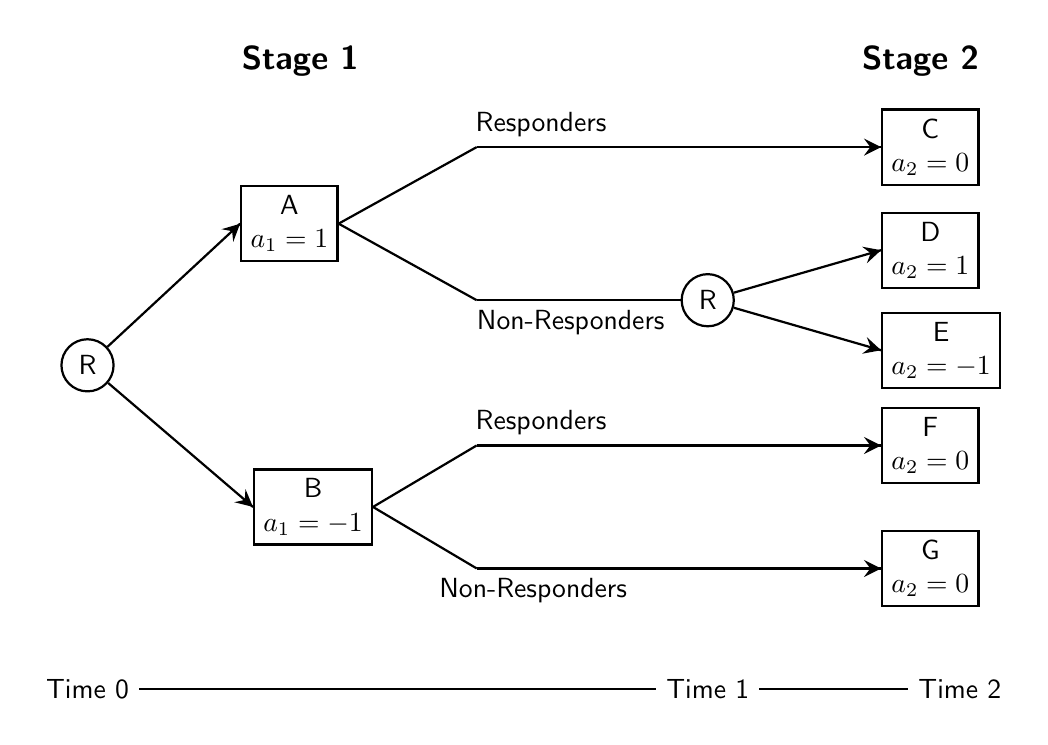
\begin{tikzpicture}[%
		node distance=6mm,
		randomize/.style={
			circle,
			minimum size=6mm,
			thick,
			black,
			draw
		},
		rerand/.style={
			xshift = 15mm
		},
		treatment/.style={
			rectangle,
			minimum size = 7mm,
			thick,
			black,
			anchor=west,
			align=center,
			draw
		},
		blank/.style={
			rectangle,
			minimum size=2mm
		},
		subgroup/.style={
			rectangle,
			rounded corners=1.5mm,
			thin,
			minimum size=6mm,
			black,
			draw
		},
		rlabel/.style={
%			font=\footnotesize,
			above,
			xshift=1mm,
			align=center
		},
		nrlabel/.style={
%			font=\footnotesize,
			below,
			xshift=-1mm,
			align=left
		},
		trialarrow/.style={
			thick,
			decoration={markings,mark=at position 1 with  {\arrow[scale=1.5,>=stealth]{>}}},
			postaction={decorate}
		},
		subsetarrow/.style={
			thin,
			decoration={markings,mark=at position 1 with {\arrow[scale=1.2,>=stealth]{>}}},
			postaction={decorate}
		}, thick]
						
		\matrix[row sep=-2mm,column sep=12mm] { %
			& \node [align=center,xshift=6mm] {\large \textbf{Stage 1}}; & & & \node [align=center,xshift=5mm] {\large \textbf{Stage 2}}; \\[5mm]
			
			% DESIGN III
			
			\node (designIII) [blank] {}; & & \node (b1-III) [blank] {}; & \node (b2-III) [blank] {}; & \node (C-III) [treatment] {C \\ $a_{2} = 0$}; \\
			& \node (stage1align) [treatment,white] {A}; & & & \\
			& & & & \node (D-III) [treatment] {D \\ $a_{2} = 1$}; \\
			& & \node (b3-III) [blank] {}; & \node (R2-III) [randomize, rerand] {R}; & \\
			& & & & \node (E-III) [treatment] {E \\ $a_{2} = -1$}; \\
			\node [randomize,white] {}; & & & &; \\	
			& & \node (b4-III) [blank] {}; & \node (b5-III) [blank] {}; & \node (F-III) [treatment] {F \\ $a_{2} = 0$}; \\
			& \node (B-III) [treatment] {B \\ $a_{1} = -1$}; & & & \\
			& & \node (b6-III) [blank] {}; & \node (b7-III) [blank] {}; & \node (G-III) [treatment] {G \\ $a_{2} = 0$}; \\[1cm]
			
			% TIMEPOINTS
			
			\node (time0) [align=center, anchor=center] {Time 0};& & & \node (time1) [align=center, anchor=center, xshift=15mm] {Time 1}; & \node (time2) [align=center, xshift = 10mm] {Time 2}; \\
		};
	
%		\draw[dashed,lightgray] (time1.north) -- (R2-III.south);
%		\draw[dashed,lightgray] (R2-III.north) -- (R3-II.south);
%		\draw[dashed,lightgray] (R3-II.north) --++(90:3.2cm);
%		
%		\draw[dashed,lightgray] (time2.north west) --++(90:33cm);
	
	
		% DESIGN III LINES
		
		\draw let \p1 = (stage1align.north), \p2=($(C-III) !.5! (R2-III)$) in node[treatment] at (\x1-15, \y2) (A-III) {A \\ $a_{1} = 1$};
		
		\draw let \p1 = (designIII.north), \p2=($(A-III.north) !.5! (B-III.south)$) in node[randomize] at (\x1, \y2) (R1-III) {R};
		
		\draw[trialarrow] (R1-III) -- (A-III.west);
		\draw (A-III.east) -- (b1-III.center);
		\draw (A-III.east) -- (b3-III.center);
		\draw (b1-III.center) -- node [rlabel] {Responders} (b2-III.center);
		\draw (b3-III.center) -- node [nrlabel] {Non-Responders} (R2-III);
		\draw[trialarrow] (b2-III.center) -- (C-III);
		\draw[trialarrow] (R2-III) -- (D-III.west);
		\draw[trialarrow] (R2-III) -- (E-III.west);
		
		\draw[trialarrow] (R1-III) -- (B-III.west);
		\draw (B-III.east) -- (b4-III.center);
		\draw (B-III.east) -- (b6-III.center);
		\draw (b4-III.center) -- node [rlabel] {Responders} (b5-III.center);
		\draw[trialarrow] (b5-III.center) -- (F-III);
		\draw (b6-III.center) -- node [nrlabel,align=center,xshift=1mm] {Non-Responders} (b7-III.center);
		\draw[trialarrow] (b7-III.center) -- (G-III.west);
			
		% TIME LINES
		
		\draw (time0) -- (time1) -- (time2);
\end{tikzpicture}
\end{document}